%\noindent
%{\bf Introduction and EFT analysis} \\
In this section we perform a collider study of the Higgs-strahlung process, $pp \to Z(\ell^+ \ell^-)h(b\bar 
b)$ in the Standard Model Effective Field Theory (SMEFT) framework. We will see that the leading high energy contribution to the $pp \to Zh$ process comes from the four 
contact interactions  $hZ_\mu \bar{u}_{L,R} \gamma^\mu u_{L,R}$ and $hZ_\mu \bar{d}_{L,R} \gamma^\mu 
d_{L,R}$ that appear in the dimension-6 Lagrangian. These are the same four EFT directions, the so called ``high 
energy primaries'' that control  high energy $Wh,~WW$ and $WZ$ production (see Ref.~\cite{Franceschini:2017xkh}). The (pseudo-)observables involved in these di-boson processes (anomalous TGCs and $Z$-pole observables)  have already been constrained at LEP.  We show in this note that    because of the higher  energies accessible at the LHC one can obtain bounds on these observables that are at least an order of magnitude stronger than those obtained at LEP.


The vertices in the dimension 6 Lagrangian that contribute 
to the $ff \to Vh$ (where $V=W,Z$) process in unitary gauge are as follows, 
\begin{eqnarray}
&&\Delta {\cal L}_6\supset \sum_f {\delta g^Z_{f}} Z_\mu \bar{f} \gamma^\mu f +\delta g^W_{ud} (W^+_\mu \bar{u}_L \gamma^\mu d_L+h.c.)
+ {g^h_{VV}}\,  h \left[W^{+\, \mu} W^-_\mu+\frac{1}{2c_{\theta_W}^2}Z^\mu Z_\mu\right]\nonumber \\
&&+  \delta g^h_{ZZ}\, h \frac{Z^\mu Z_\mu}{2c_{\theta_W}^2} + \sum_f g^h_{Zf}\,\frac{h}{v}Z_\mu \bar{f} \gamma^\mu f+g^h_{Wud}\,\frac{h}{v}(W^+_\mu \bar{u}_L \gamma^\mu d_L+h.c.)
+{\kappa_{Z \gamma }}\frac{h}{v} A^{\mu\nu} Z_{\mu\nu} \nonumber \\ 
&&+\kappa_{WW}\,\frac{h}{v}
 W^{+\, \mu\nu}W^-_{\mu\nu}
+\kappa_{ZZ}\,\frac{h}{2v} Z^{\mu\nu}Z_{\mu\nu}\,.
\label{lagr}
\end{eqnarray}
Here we have used the Lagrangian presented in Ref.~\cite{Gupta:2014rxa, Pomarol:2014dya}, where $\alpha_{em}$, $m_Z$ and $m_W$   have been used as input parameters and any corrections 
to the SM vector boson propagators  have 
been traded in favour of the vertex corrections. After summing over all $V$-polarisations, the leading 
piece in the high energy cross-section deviation for $ff \to Vh$ , is proportional to the four  contact interactions:  $g^h_{Zf}$, with $f=u_L, u_R,d_L$ and $d_R$.\footnote{There exists a basis independent constraint at the dimension-6 level, $\sqrt{2}\;g^h_{Wud}= (g^h_{Zd_L}-g^h_{Zu_L})$. } Table~\ref{dirn}, shows the linear combinations of Wilson coefficients contributing to the four 
$g^h_{Zf}$ couplings in different EFT bases.  The aforementioned directions are shown in the BSM Primary basis of Ref.~\cite{Gupta:2014rxa}, 
where the Wilson coefficients are already constrained pseudo-observables. In this basis we see that these can be written in terms of already constrained LEP (pseudo)observables. 

Given the inability to control the polarisation of the initial state partons in a hadron collider, 
the process, in reality, only probes two of the above four directions. Taking only the interference 
term, we find these directions to be
\begin{equation}
g^Z_{\textbf{u}}= g^h_{Zu_L}+\frac{g^Z_{u_R}}{g^Z_{u_L}} g^h_{Zu_R},\; 
g^Z_{\textbf{d}}= g^h_{Zd_L}+\frac{g^Z_{d_R}}{g^Z_{d_L}} g^h_{Zd_R}\,.
\end{equation}
 %where $g^Z_f$ is defined below \eq{amps}. 
 At a given energy, a linear combination of the up-type and down-type coupling 
 deviations, enters the interference term for the 
 $pp \to Zh$ process, $g^Z_{\textbf{p}}= g^Z_{\textbf{u}}+ \frac{{\cal L}_d(\hat{s})}{{\cal L}_u(\hat{s})}g^Z_{\textbf{d}},$
where ${\cal L}_{u,d}$ is the $u \bar{u}$, $d \bar{d}$ luminosity at a given partonic centre of mass 
energy. The luminosity ratio changes very little with energy: between 0.65 and 0.59 as 
$\sqrt{\hat{s}}$ is varied from 1 to  2 \UTeV. Thus, to a good approximation, $pp \to Zh$ probes 
the single direction, 
\begin{equation}
g^Z_{\textbf{p}}=g^h_{Zu_L} -0.76~g^h_{Zd_L}   - 0.45~g^h_{Zu_R} + 0.14~g^h_{Zd_R}  \,.
\label{compdir}
\end{equation}
%where we have substituted the values for $g^Z_f$ and evaluated the luminosities at the energy 
using ${\hat{s}}=(1.5~\text{\UTeV})^2$. Using Tab.~\ref{dirn}, one can now write this in terms of the LEP-constrained pseudo-observables,
\begin{eqnarray}
g^h_{Z\textbf{p}}&=&2~\delta g^h_{Zu_L} -1.52~\delta g^h_{Zd_L}   - 0.90~\delta g^h_{Zu_R} + 0.28~\delta g^h_{Zd_R}\nonumber\\
&&-0.14~\delta \kappa_\gamma   -0.89~\delta g^Z_1 \nonumber\\
g^h_{Z\textbf{p}}&=&-0.14~(\delta \kappa_\gamma-\hat{S}+Y) -0.89~\delta g^Z_1  -1.3~W
\label{diru}
\end{eqnarray}
where the first  and second lines apply respectively to the general and universal case (third and fourth row of Table~\ref{dirn}). 
 
%%%%%%%%%%%%%%%%%%%%%%%%%%%%%%%%%%%
\begin{table*}[!t]
\begin{center}
\small
\begin{tabular}{|c|c|}%\hline
\hline
&EFT directions probed by high energy $ff \to Vh$ production \\
\hline
\hline
 Warsaw Basis~\cite{Grzadkowski:2010es} & $- \frac{2 g}{c_{\theta_W}}\frac{v^2}{\Lambda^2}(|T_3^f|c^{1}_L-T_3^f c^{3}_L+(1/2-|T_3^f|)c_f)$\\
BSM Primaries~\cite{Gupta:2014rxa} &$   \frac{2 g}{c_{\theta_W}}Y_f t_{\theta_W}^2 \delta \kappa_\gamma+2 \delta g^Z_{f}- \frac{2 g}{c_{\theta_W}}(T^f_3 c_{\theta_W}^2 + Y_f s_{\theta_W}^2)\delta g_1^Z $\\
 SILH Lagrangian~\cite{Giudice:2007fh} &$  \frac{g}{c_{\theta_W}}\frac{m_W^2}{\Lambda^2}(2 |T_3^f|\hat{c}_W-2t_{\theta_W}^2 Y_f \hat{c}_B)$\\
 Universal observables &$ \frac{2 g}{c_{\theta_W}}Y_f t_{\theta_W}^2  (\delta \kappa_\gamma-\hat{S}+Y)- \frac{2 g}{c_{\theta_W}}(T^f_3 c_{\theta_W}^2 + Y_f s_{\theta_W}^2)\delta g_1^Z- \frac{2 g}{c_{\theta_W}}T^f_3 W$\\
 High Energy Primaries~\cite{Franceschini:2017xkh} &$ -\frac{2 m_W^2}{g c_{\theta_W} }(|T_3^f| a_q^{(1)}-T_3^f a_q^{(3)}+(1/2-|T_3^f|)a_f)$\\
\hline
 \end{tabular}
  \caption{ The linear combinations of Wilson coefficients contributing to the contact interaction couplings $g^h_{Zf}$where  $f=u_L, d_L, u_R, d_R$. the direction for a given $f$  can  be read off from this table by substituting the corresponding  value of the $SU(2)_L$ and $U(1)_Y$ quantum numbers  $T_3^f$ and $Y_f$. Here $\hat{c}_W=c_W+c_{HW}-c_{2W}$ and $\hat{c}_B= c_B+c_{HB}-c_{2B}$. For the nomenclature of the operators, their corresponding Wilson coefficients and observables see for eg. Ref.~\cite{Franceschini:2017xkh}.}
  \label{dirn}
\end{center}
\end{table*}

%%%%%%%%%%%%%%%%%%%%%%%%%%%%%%%%%%

To estimate  the cut-off for 
our EFT, note that the ${g}^h_{Vf}$ couplings arise from current-current operators that can be generated, for instance, 
by integrating out at tree-level a heavy $SU(2)_L$ triplet (singlet) vector $W'^a$ ($Z'$) that couples 
to SM fermion currents, $\bar{f} \sigma^a \gamma_\mu f$ ($\bar{f} \gamma_\mu f)$ with a coupling 
$g_f$ and to the Higgs current $i{H}^\dagger \sigma^a \lra{D}_\mu H$ ($i{H}^\dagger \lra{D}_\mu H$) 
with a coupling $g_H$. This gives ${g}^h_{Zf}\sim g_H g g_f v^2/\Lambda^2$,
where $\Lambda$ is the mass of the massive vector and thus the cut-off for our EFT description. A universal coupling to the SM fermions can arise  
via kinetic mixing of the heavy vector with the SM gauge bosons; this would give $g_f=g/2$ ($g_f=g' Y$), such that,
\begin{equation}
  \label{cutoff}
{g}^h_{Zu_L,d_L} \sim \frac{g_H g^2  v^2}{ 2\Lambda^2},\;
{g}^h_{Zu_R,d_R} \sim \frac{g_H g g' Y_{u_R,d_R} v^2}{\Lambda^2}.
\end{equation}
 For a given  set of couplings   $\{{g}^h_{Zu_L} ,{g}^h_{Zd_L} ,{g}^h_{Zu_R} ,{g}^h_{Zd_R} \}$, the cut-off is  evaluated using 
 Eq.~\ref{cutoff} with $g_H=1$ (note that this is somewhat larger than the value corresponding to the SM $hZZ$ coupling) and taking the smallest of the four values. \\ \\
 
                                                                                                                
% %%%%%%%%%%%%%%%%%%%%%%%%%%%%%%%%%%%                                                                                                              
%\noindent
%{\bf Collider Analysis}\\
For our collider analysis, we consider  $Z(\ell^+\ell^-)h$ production from a pair of quarks as well as from a 
pair of gluons.  For the decay of the Higgs boson,  we find that at an integrated luminosity of  300 fb$^{-1}$,  the di-photon mode is not feasible as it yields less than 5 events at high energies ($p_{T,Z}>150$ \UGeV). We thus focus on the decay $h\to b\bar b$ to obtain large statistics. The dominant backgrounds are then  
$Zb\bar{b}$ and the irreducible $Zh$ production in SM. Reducible contributions also arise from $Z+$ jets production (where we include $c$-quarks but do not require that they are explicitly tagged). We employ the BDRS 
approach~\cite{Butterworth:2008iy} and demand a fat jet with a cone radius of $R=1.2$. More details of the Monte-Carlo analysis, the QCD corrections, the detailed cut-based 
and multivariate analyses (MVA) can be found in Ref.~\cite{Banerjee:2018bio}. Finally, we find a cut-based (MVA) SM $Zh$ to $Zb\bar{b}$ ratio of $\sim 0.26 \; 
(0.50)$.

%%%%%%%%%%%%%%%%%%%%%%%%%%%%%%%%%%%%
\begin{figure}[!t]\centering
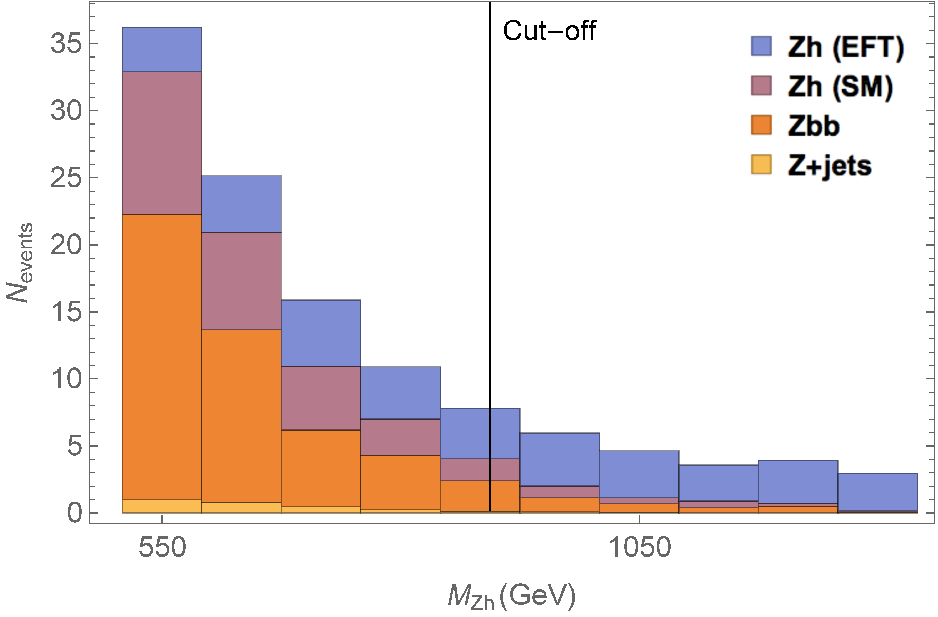
\includegraphics[width=0.45\textwidth]{\main/section4/plots/bars}
\caption{The differential distribution of events at an integrated luminosity of 300 fb$^{-1}$ with respect to $M_{Zh}$ for the EFT signal as well as the different backgrounds. The EFT signal corresponds to the point $\{{g}^h_{Zu_L} ,{g}^h_{Zd_L} ,{g}^h_{Zu_R} ,{g}^h_{Zd_R} \}=\{-0.005, 0.0001 , -0.010, 0.005 \}$ which is allowed by  LEP bounds. The vertical line shows the cut-off evaluated using Eq.~\ref{cutoff}.}
\label{bars}
\end{figure}
%%%%%%%%%%%%%%%%%%%%%%%%%%%%%%%%%%%%

To discriminate between the EFT signal and the irreducible SM $Zh(b\bar b)$ background we study  the 
growth of the EFT cross-section at high energies. This can be seen in Fig.~\ref{bars}  where we show the differential distribution with respect to $M_{Zh}$, the invariant mass of the leptons and the fat jet, for the EFT signal as well as for the different backgrounds. The EFT signal corresponds to a point that can be excluded in our analysis but is allowed by the LEP constraint.  To fully utilise the shape deviation of the EFT signal with respect to the background, 
we perform a binned log likelihood analysis assuming a 5$\%$ systematic error taking only events below the cut-off (evaluated as explained below Eq.~\ref{cutoff}). To obtain the   95$\%$ CL exclusion curve, we assume that 
the observed number of events would agree with the SM. \\ \\
%%%%%%%%%%%%%%%%%%%%%%%%%%%%%%%%%%

%\noindent
%{\bf Discussion and Conclusions}\\
%%%%%%%%%%%%%%%%%%%%%%%%%%%%%%%%%%
Taking into account only the SM-BSM interference term, we find the following per-mille level bounds for 300 (3000) fb$^{-1}$, 
\begin{equation}
g^h_{Z\textbf{p}} \in  \left[-0.004,0.004\right] \; (\left[-0.001,0.001\right])
\label{obo}
\end{equation}
The above bounds    translate to a lower bound on the scale of new physics given by 2.4 \UTeV (4.4 \UTeV) at 300 fb$^{-1}$ (3000 fb$^{-1}$) using Eq.~\ref{cutoff}.  To compare the above projections with existing LEP bounds, one can now extract bounds on the LEP observables contributing to $g^h_{Z\textbf{p}}$ in Eq.~\ref{diru} by turning them  on one by one. We show the results  in Tab.~\ref{lepb}. For the TGCs $\delta g^Z_1$ and $\delta \kappa_\gamma$, our projections are much stronger than the LEP bounds and  in the case of the $Z$-pole observables $\delta g^Z_f$, that parametrise the deviations of the $Z$ coupling to quarks, they are comparable. 

%%%%%%%%%%%%%%%%%%%%%%%%%%%%%%%%%%%%%%%%%%%%%%
\begin{figure}[!t]\centering
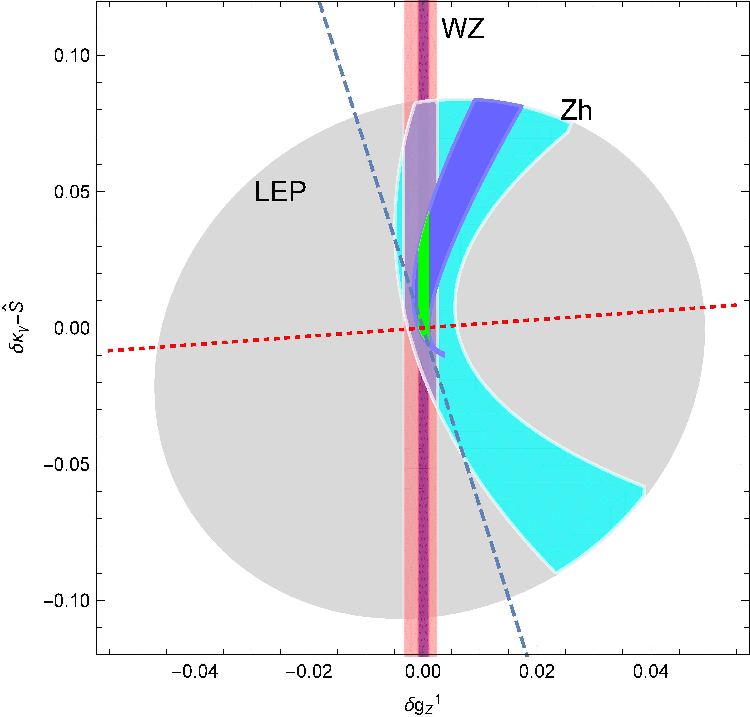
\includegraphics[width=0.45\textwidth]{\main/section4/plots/300plot}
\caption{The light blue (dark blue) region above shows the projection for the allowed region with 300 fb$^{-1}$ (3 ab$^{-1}$) data from the 
$pp \to Zh$ process  in the $\delta \kappa_\gamma-\hat{S}$ vs $\delta g^Z_1$ plane for universal models. We show in grey the allowed region after LEP bounds (taking the TGC $\lambda_\gamma=0$, a conservative choice) are imposed.  In pink (dark pink)  we show the region that corresponds to the projection from the $WZ$ process  with 300 fb$^{-1}$ (3 ab$^{-1}$) data derived in Ref.~\cite{Franceschini:2017xkh} and the purple (green) region shows the region that survives from a combination of the $Zh$ and $WZ$ projections with 300 fb$^{-1}$ (3 ab$^{-1}$) data.}\label{bounds}
\end{figure} 
%%%%%%%%%%%%%%%%%%%%%%%%%%%%%%%%%%%%

For the universal case, we perform a more detailed analysis. The results are shown in the 
$\delta \kappa_\gamma-\hat{S}$ vs. $\delta g^Z_1$ plane  in Fig.~\ref{bounds} for the interesting class of models where $W=Y=0$~\cite{Franceschini:2017xkh}. The  
direction related to the $pp \to Zh$ interference term, \textit{i.e.}, $g^h_{Z\textbf{p}}=0$ (see Eq.~\ref{compdir} and the second line of Eq.~\ref{diru}) is shown by the dashed blue line, whereas the direction orthogonal to it is shown by the dotted red line.  Once the LEP II bounds~\cite{LEP2} from the $e^+e^- \to W^+W^-$ 
process are imposed, the allowed region that remains is shown by the grey shaded area. We show the results of this work  in blue (light (dark) blue for results at
300 (3000) fb$^{-1}$).  The shape of the allowed region arises due to the fact that the interference term vanishes along the dashed blue line and the squared term increases in magnitude as we move away from the origin. This curves the allowed region away from the dashed line as we move away from the origin.  The accidental cancellation of the interference term means that our bounds are susceptible to dimension-8 effects along this direction. On the other hand our bounds are more robust and not susceptible to such effects in the orthogonal direction shown by the red dotted line.

%%%%%%%%%%%%%%%%%%%%%%%%%%%%%%%%%%
\begin{table}[t]
\begin{center}

\begin{tabular}{c|c|c}%\hline
&Our Projection &LEP Bound\\\hline
$\delta g^Z_{u_L}$         & $\pm0.002~(\pm0.0007)$ & $-0.0026\pm 0.0016$\\
$\delta g^Z_{d_L}$         & $\pm0.003~(\pm0.001)$  & $0.0023\pm 0.001$\\
$\delta g^Z_{u_R}$         & $\pm0.005~(\pm0.001)$  & $-0.0036\pm 0.0035$\\
$\delta g^Z_{d_R}$         & $\pm0.016~(\pm0.005)$  & $0.0016\pm 0.0052$\\
$\delta g^Z_1$             & $\pm0.005~(\pm0.001)$  & $0.009^{+0.043}_{-0.042}$\\
$\delta \kappa_\gamma$     & $\pm0.032~(\pm0.009)$  & $0.016^{+0.085}_{-0.096}$\\
$\hat{S}$                  & $\pm0.032~(\pm0.009)$ & $0.0004 \pm 0.0007$\\
$W$                        & $\pm0.003~(\pm0.001)$  & $0.0000 \pm 0.0006$\\
$Y$                        & $\pm0.032~(\pm0.009)$  & $0.0003\pm 0.0006$
 \end{tabular}
  \caption{Comparison of the bounds obtained in this work with existing LEP bounds obtained by turning on the LEP observables in Eq.~\ref{diru} one by one and using Eq.~\ref{obo}. The LEP bounds on the $Z$ coupling to quarks has been obtained from Ref.~\cite{Falkowski:2014tna}, the bound on the TGCs from Ref.~\cite{LEP2}, the bound on $\hat{S}$ from Ref.~\cite{Baak:2012kk} and  finally the bounds on $W,Y$ have been obtained from Ref.~\cite{Barbieri:2004qk}. Except for the case of the bounds on $\delta g^Z_f$, all of the bounds in the last column were derived by turning on only the given parameter and putting all other parameters  to zero. The numbers outside (inside) brackets, 
  in the second column, denote our bounds with $\mathcal{L} = 300 \; (3000)$ fb$^{-1}$.  \label{lepb}}
\end{center}
\end{table}
%%%%%%%%%%%%%%%%%%%%%%%%%%%%%%%%%%

As $VV$ production constrains the same set of operators as the $Vh$ 
production in Fig.~\ref{bounds}, we also show the projected bound from the $WZ$ process at 300 
fb$^{-1}$ obtained in Ref.~\cite{Franceschini:2017xkh} (see section~\ref{WZlong}). Only the 
purple region remains when both these bounds are combined  at 300 fb$^{-1}$. This shrinks further to the green region  at 3000 fb$^{-1}$. A drastic reduction in the allowed LEP region is   thus possible by considering the $pp \to Zh$ at high energies.

